\documentclass{report}

%%% Imports %%%
% \usepackage[Lenny]{fncychap}
\usepackage{multicol}
\setlength{\columnseprule}{1pt}
\setlength{\columnsep}{1cm}
\usepackage[utf8]{inputenc}
\usepackage{XCharter}
\usepackage{float}
\usepackage[T1]{fontenc}
\usepackage{textcomp}
\usepackage[english]{babel}
\usepackage{amsmath, amssymb, amsthm}
\usepackage[a4paper, total={7.5in,10in}]{geometry}
\usepackage{blindtext}
\usepackage{hyperref}
\usepackage{graphicx}
\usepackage{empheq}
\usepackage{mdframed}
\usepackage{booktabs}
\usepackage{color}
\usepackage{psfrag}
\usepackage{bm}
\usepackage{tcolorbox}
\usepackage{bookmark}
\usepackage{tikz}
\newcommand{\warning}{
	{\fontencoding{U}\fontfamily{futs}\selectfont\char 66\relax}
}
\setlength{\parindent}{0em}
\usepackage{silence}
%Disable all warnings issued by latex starting with "You have..."
\WarningFilter{latex}{You have requested package}
%Code listing env
\usepackage{listings}
\usepackage{rust_latex/listings-rust}
\usepackage{xcolor}

\definecolor{codegreen}{rgb}{0,0.6,0}
\definecolor{codegray}{rgb}{0.5,0.5,0.5}
\definecolor{codepurple}{rgb}{0.58,0,0.82}
\definecolor{backcolour}{rgb}{0.95,0.95,0.92}

\lstdefinestyle{mystyle}{
		backgroundcolor=\color{backcolour},   
		commentstyle=\color{codegreen},
		keywordstyle=\color{magenta},
		numberstyle=\tiny\color{codegray},
		stringstyle=\color{codepurple},
		basicstyle=\ttfamily\footnotesize,
		breakatwhitespace=false,         
		breaklines=true,                 
		captionpos=b,                    
		keepspaces=true,                 
		numbers=left,                    
		numbersep=5pt,                  
		showspaces=false,                
		showstringspaces=false,
		showtabs=false,                  
		tabsize=2
}

\lstset{style=mystyle}

%%% Inkscape Integration %%%
\usepackage{import}
\usepackage{pdfpages}
\usepackage{transparent}
\usepackage{xcolor}

\newcommand{\incfig}[2][1]{%
		\def\svgwidth{#1\columnwidth}
		\import{./figures/}{#2.pdf_tex}
}

\pdfsuppresswarningpagegroup=1

%%% Define colors %%%%
\definecolor{Green}{rgb}{0.2,0.9,0.2}

%%% Title and author %%%
\author{Damian Hubert}
\title{Rust - Level 1}
%%% Main Document Space %%%
\begin{document}

\maketitle
\tableofcontents


\chapter{Fondamentals}

\begin{multicols*}{2}


\section{Cargo}
\begin{itemize}
	\item Package manager, Build system, Test runner, Docs generator
\end{itemize}

\begin{tcolorbox}[title=Creating Project,colback=backcolour,size=small,left=4mm]
\begin{lstlisting}[language=bash]
cargo new "app name"
\end{lstlisting}
\end{tcolorbox}

\begin{itemize}
	\item \textbf{Cargo.toml} is the config file for the project
		\begin{itemize}
			\item \textbf{name} is independent of the directory name 
			\item \textbf{version} uses semantic versioning, see \href{https://semver.org}{this link} 
			\item \textbf{authors} should be completed by itself using git credentials 
		\end{itemize}
	\item \textbf{src} subdirectory with \textbf{main.rs} 
\end{itemize}

\begin{tcolorbox}[title=Running a Program,colback=backcolour,size=small,left=4mm]
\begin{lstlisting}[language=bash]
cargo run
\end{lstlisting}
\end{tcolorbox}

\textbf{Target directory}
\begin{itemize}
	\item Where cargo outputs all its build artefacts 
	\item \textbf{To add in .gitignore} 
\end{itemize}

By default, cargo compiles the project with debug symbols
\begin{tcolorbox}[title=Disable Debug Symbols,colback=backcolour,size=small,left=4mm]
\begin{lstlisting}[language=bash]
cargo run --release
# will be a lot faster
\end{lstlisting}
\end{tcolorbox}


\section{Variables}

\subsection{Default}

\begin{tcolorbox}[title=Structure,colback=backcolour,size=small,left=4mm]
\begin{lstlisting}[language=rust]
fn main() {
	let whatever = 2;
	// auto
	let whatever: i32 = 2;
	// specific type
}
\end{lstlisting}
\end{tcolorbox}

\begin{itemize}
	\item \textbf{let} declares a variable 
	\item Rust is a \textbf{strongly typed} language
		\begin{itemize}
			\item By default it will be \textbf{auto} 
			\item But a \textbf{specific} type can be specified
		\end{itemize}
\end{itemize}

\begin{itemize}
	\item \textbf{let} statements can also initialize \textbf{multiple} variables at once, it can \textbf{de-structure} the data
\end{itemize}

\begin{tcolorbox}[title=Deconstruction Example,colback=backcolour,size=small,left=4mm]
\begin{lstlisting}[language=rust]
fn main() {
	let (hello, world) = (8, 50);
}
\end{lstlisting}
\end{tcolorbox}

\subsection{Immutability}

\begin{itemize}
	\item By default, variables are \textbf{immutable} 
		\begin{itemize}
			\item \textbf{To make it mutable} add \textbf{mut} after let
		\end{itemize}
\end{itemize}

\subsection{Constants}

\begin{itemize}
	\item \textbf{const} instead of let
		\begin{itemize}
			\item The \textbf{convention} is to use\\ 
        SCREAMING\_NAMES 
			\item The type annotation is \textbf{required} here !
		\end{itemize}
	\item \textbf{Two reasons} to use const
		\begin{enumerate}
			\item A const is \textbf{global}  
			\item They're really \textbf{fast} at compile time
		\end{enumerate}
\end{itemize}


\section{Scope}

\begin{itemize}
	\item The scope is the place in the code where we are allowed to use the variables 
	\item The scope of variables is contained inside its block, and sub-blocks. If a block ends : the variable is \textbf{immediately dropped} 
	\item Variables can be \textbf{shadowed}, they're always \textbf{local to their scope}  
\end{itemize}

\begin{tcolorbox}[title=Shadowing,colback=backcolour,size=small,left=4mm]
\begin{lstlisting}[language=rust]
fn main() {
	let x = 5;
	{
		let x = 99;
		println!("{}", x); // prints 99
	}
	println!("{}", x); // print 5
}
\end{lstlisting}
\end{tcolorbox}

\begin{tcolorbox}[title=Shadowing in the same scope,colback=backcolour,size=small,left=4mm]
\begin{lstlisting}[language=rust]
let mut x = 5;
let x = x; // is now immutable
// can also modify the type of the variable
\end{lstlisting}
\end{tcolorbox}


\section{Memory Safety}
\begin{itemize}
	\item The \textbf{compiler} must be sure that all variables will have a value assigned to it
\end{itemize}


\section{Functions}

\begin{itemize}
	\item Naming convention : \textbf{sneak\_cases}
\end{itemize}

\begin{tcolorbox}[title=Functions doesn't have to appear before we call them,colback=backcolour,size=small,left=4mm]
\begin{lstlisting}[language=rust]
fn main() {
	do_stuff();
}
fn do_stuff() {
}
// is valid !
\end{lstlisting}
\end{tcolorbox}

\begin{itemize}
	\item Functions \textbf{parameters} are defined with \textbf{(name: type,..)} 
	\item Specify the \textbf{return type} by adding \textbf{-> type}  
\end{itemize}

\begin{tcolorbox}[colback=backcolour,size=small,left=4mm]
\begin{lstlisting}[language=rust]
fn do_stuff(qty: f64, oz: f64) -> f64 {
	return qty * oz;
	// The short hand for returning values is to leave the ";" off
	qty * oz
}
\end{lstlisting}
\end{tcolorbox}

\begin{itemize}
	\item Leaving the ";" off the last expression in a block, will make it be returned as the value of the block
	\item There isn't support for named arguments, so all the values must be provided in the \textbf{correct order}
	\item A single function doesn't support \textbf{variable} number of arguments or $\not =$ types for the same arguments
		\begin{itemize} 
			\item But macro such as \textbf{println!} do ! 
			\item The name of a macro always end with a "!"
		\end{itemize}
\end{itemize}

\section{Module System}

We create a library called \textit{lib.rs} 

\begin{tcolorbox}[title=,colback=backcolour,size=small,left=4mm]
\begin{lstlisting}[language=rust]
hello
--Cargo.toml
--src
  -- lib.rs // the hello library
  -- main.rs // the hello binary
\end{lstlisting}
\end{tcolorbox}

\begin{tcolorbox}[title=In lib.rs,colback=backcolour,size=small,left=4mm]
\begin{lstlisting}[language=rust]
fn greet() {
  println!("Hi");
}
\end{lstlisting}
\end{tcolorbox}

\begin{tcolorbox}[title=To call it in main.rs,colback=backcolour,size=small,left=4mm]
\begin{lstlisting}[language=rust]
fn main() {
  hello::greet(); //absolute path, wont work yet
  }
// because all items in a library are private by default
--> pub fn...
\end{lstlisting}
\end{tcolorbox}

\begin{itemize}
  \item \textbf{Absolute path} is library name (same as project), here : \textit{hello}, + scope operator :: and then name of the function 
  \item We need to add \textbf{pub} in front of the function 
  \item Absolute path are \textbf{very long} so \textit{use} comes in handy
\end{itemize}

\begin{tcolorbox}[title=use,colback=backcolour,size=small,left=4mm]
\begin{lstlisting}[language=rust]
// in main
use hello::greet;
// brings greet into scope for all of main
// hello::greet becomes greet

//we can call the Standard Library with
use std::collection::HashMap; // example
// Always available
\end{lstlisting}
\end{tcolorbox}

When things are \textbf{not in the std}, we search on \textbf{crates.io}, crate $\equiv$ package,
\textbf{import} it in Cargo.toml

\begin{tcolorbox}[title=Cargo.toml,colback=backcolour,size=small,left=4mm]
\begin{lstlisting}[language=rust]
[dependencies]
pack_name = "0.2.6"
\end{lstlisting}
\end{tcolorbox}

\end{multicols*}

\chapter{Primitive Types and Control Flow}

\begin{multicols*}{2}

\section{Scalar Types}

\begin{itemize}
  \item \textbf{Integers}
    \begin{itemize}
      \item \textbf{unsigned} starts with \textbf{u}, \textbf{signed} with \textbf{i} 
      \item they are \textbf{followed by} the number of bits the integer as $2^{3 \rightarrow 7}$ 
      \item Exception made for \textbf{usize} which is the size of the platform pointer type and can represent
        every memory address in the process; vectors and arrays usually use it to index 
      \item All types are not supported on all hardware 
      \item Int can be \textbf{specified} in a lot of ways : decimal, [0x]hex, [0o]octal, [0b]binary and byte(u8 only)[b'<utf-8 char>']
      \item They can have any number of "\_" in them, for \textbf{convenience} 
    \end{itemize}
  \item \textbf{Float} 
    \begin{itemize}
      \item Much simpler : f32, \textbf{f64} : the \textbf{default}, more precise but can be really slow on $<$ 64bit architecture 
      \item Floating point literals follow the \textbf{IEEE-754} std, we write them like \textit{3.14159} 
    \end{itemize}
  \item \textbf{Booleans} 
    \begin{itemize}
      \item \textbf{bool} can be \textbf{true} or \textbf{false} 
      \item \textbf{arithmetic} wont work unless casted like "true as u8"
    \end{itemize}
  \item \textbf{Characters}
    \begin{itemize}
      \item \textbf{char} are always \textbf{4 bytes} -> an array of chars are always UCS-4 / UTF-32 string 
      \item Fairly useless because string are UTF-8 
      \item let my\_letter = '<anything, unicode>';
    \end{itemize}
\end{itemize}

\begin{tcolorbox}[title=Suffixe variable type,colback=backcolour,size=small,left=4mm]
\begin{lstlisting}[language=rust]
let x: u16 = 5;
// suffix the literal with the wanted type works too
let x: 5u16; // useful when passing a literal to a generic function that could accept multiple numeric types
let x: 5_u16;
\end{lstlisting}
\end{tcolorbox}

\section{Compound Types}

  They gather \textbf{multiple values of other types into one}

\begin{itemize}
  \item $\diamond$ \textbf{Tuple} stores multiple values of \textbf{any type} 
  \item let info = (1, 3.3, 999); 
  \item \textbf{type annotation} : let info: (u8, f64, i32) = (1, 3.3, 999); 
  \item Two ways to \textbf{access members} :
    \begin{enumerate}
      \item \textbf{dot syntax} : let jets = info.0; 
      \item \textbf{all at once} : let (jets, fuel, ammo) = info; \textbf{max 12 arity} 
      \item \textbf{arity} is the number of elements
    \end{enumerate}
  \item $\diamond $ \textbf{Arrays} elements in contrast has to have to \textbf{same type} 
  \item let buf = [1, 2, 3]; 
  \item let buf = [0; 3]; : value; number 
  \item let buf: [u8; 3] = [1, 2, 3]; 
  \item \textbf{Indexation} : buf[0], array are \textbf{limited} to a size of \textbf{32} 
  \item Arrays lives on the \textbf{stack by default} and are \textbf{fixed size} so we'll usually use \textbf{Vec} 
\end{itemize}

\section{Control Flow}

\subsection{If expression}%
\label{sub:If expression}

\begin{itemize}
  \item Does not need () around the condition
  \item The condition \textbf{must} evaluate to a boolean, rust does not like \textbf{type coercion} 
  \item An \textbf{expression} means that it \textbf{returns a value}, \textbf{unlike statements} 
\end{itemize}

\begin{tcolorbox}[title=If,colback=backcolour,size=small,left=4mm]
\begin{lstlisting}[language=rust]
if num == 5 {  
  msg = "five";
} else if num == 4 {
  msg = "four";
} else {
  msg = "other";
}
// or
msg = if num == 5 {  //everything between if and { will be the condition
  "five" // ; are left off to the value get's returned like tail expressions
} else if num == 4 {
  "four"
} else {
  "other"
}; // only necessary when we use the value of an if expression
// cannot use return, it only applies to function bodies
// all the blocks return the same type

//one line
num = if a {b} else {c};
\end{lstlisting}
\end{tcolorbox}

\subsection{Loops}%
\label{sub:Loops}

\begin{itemize}
  \item If the compilers knows a loop is \textbf{unconditional} there are some cool optimizations 
  \item by itself \textcolor{blue}{continue} and \textcolor{blue}{break} will affect their inner loop
\end{itemize}

\begin{tcolorbox}[title=Unconditional Loop,colback=backcolour,size=small,left=4mm]
\begin{lstlisting}[language=rust]
'bob: loop { // 'bob is a loop annotation
  loop {
    loop {
      break 'bob; //we use the annotation to break out of a specific loop
    }
  }
}
// continue follows the same structure
\end{lstlisting}
\end{tcolorbox}

\begin{itemize}
  \item While loop are conditional except they also \textbf{terminate} the loop when the condition eval to false
\end{itemize}

\begin{tcolorbox}[title=While Loops,colback=backcolour,size=small,left=4mm]
\begin{lstlisting}[language=rust]
while dizzy() { // has to be boolean
  // do stuff
}

//is equivalent to  

loop{
  if !dizzy() { break }
  // do stuff
}

// do while are easy to do
loop{
  // do stuff
  if !dizzy() { break }
}
\end{lstlisting}
\end{tcolorbox}

\subsection{For Loops}%
\label{sub:For .. in range}

\begin{tcolorbox}[title=For Loops,colback=backcolour,size=small,left=4mm]
\begin{lstlisting}[language=rust]
for num in [7,8,9].iter() {
  // do stuff with num
}
// the iterator we use determines the items we take and their order 
// we can stack methods like map, filter and fault

// for loops can use pattern to unpack the items they receive
for (x, y) in array.iter() {
  // do stuff with x and y
}

// in range loops
for num in 0..50 { // [i..n[
for num in 0..=50 { // [i..n]
  // do stuff with num
}

\end{lstlisting}
\end{tcolorbox}

\section{Strings}

6 types in the rust std but only 2 are \textbf{important} and \textbf{overlap} each other

\begin{itemize}
  \item \textcolor{red}{\&}\textcolor{cyan}{str} : \textcolor{red}{borrowed} \textcolor{cyan}{string slice} often refers to a string
    which is confusing because the other string type is a \textcolor{blue}{String}  
  \item A litteral string is always a \&str 
  \item The biggest $\neq$ being that the \&str \textbf{cannot be modified} while the \textbf{String can} 
\end{itemize}

\begin{tcolorbox}[title=Creating String,colback=backcolour,size=small,left=4mm]
\begin{lstlisting}[language=rust]
let msg = "ab<unicode>".to_string(); // to create a string from a borrowed string slice
// or by passing a bss to String::from
let msg = String::from("ab<unicode>");
\end{lstlisting}
\end{tcolorbox}
\begin{figure}[H] 
	 \centering 
	 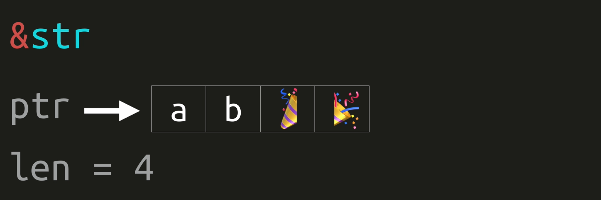
\includegraphics[width=2in]{screenshots/2022-07-15T23-25-31Z.png} 
   \caption{Are made out of a pointer to some bytes, a length, is a \textbf{subset} of a \textbf{string} }
 \end{figure}

 \begin{figure}[H] 
	 \centering 
	 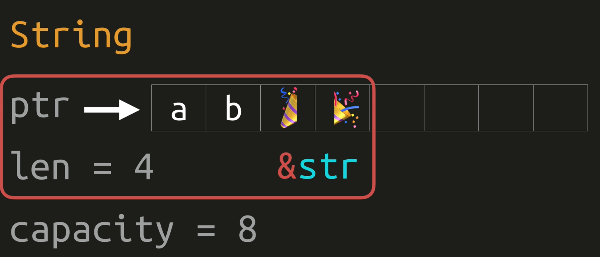
\includegraphics[width=2in]{screenshots/2022-07-15T23-28-08Z.png} 
	 \caption{Are made out of a pointer to some bytes, a length \textbf{and a capacity} that may vary upwards} 
 \end{figure}

\begin{itemize}
  \item \textbf{Both} are \textbf{valid UTF-8} by definition, compiler enforcement and runtime checks 
  \item Strings cannot be indexed by character position $\rightarrow$ lots of languages, some unicode
    takes more than a byte, a UTF-8 char can be represented by up to 4 bytes ! Diacritics are unicode that combines,
    we are searching for graphemes 
  \item Because rust emphasize on speed, indexing operations on std library collections are guaranteed to be constant time,
    this does not work with strings
\end{itemize}

\begin{tcolorbox}[title=When presented with a string,colback=backcolour,size=small,left=4mm]
\begin{lstlisting}[language=rust]
word.bytes(); //to access the vector of UTF-8 bytes, which can be indexed because bytes are fixed size
// works fine for English, without ASCII
word.chars(); //to get a iterator to iterate through Unicode scalars

unicode-segmentation !package! // providing functions that returns iterators handling graphemes 
graphemes(my_string, true)

// those solution guarantee a constant time operation
\end{lstlisting}
\end{tcolorbox}

\begin{figure}[H] 
	 \centering 
	 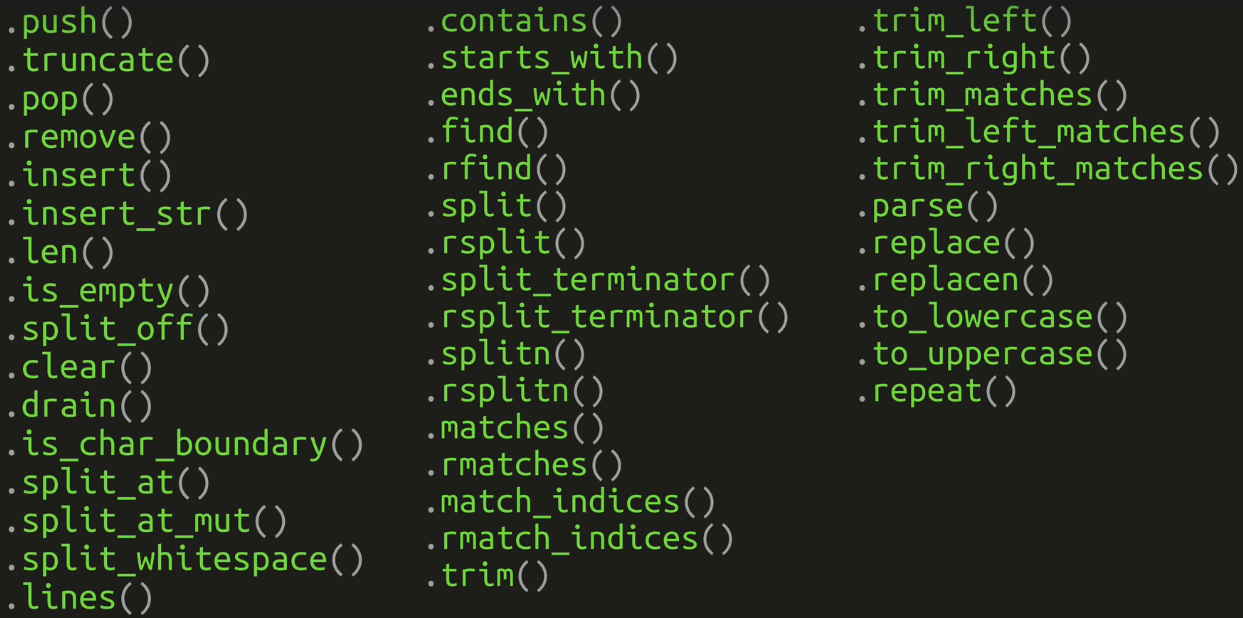
\includegraphics[width=2.8in]{screenshots/2022-07-15T23-46-36Z.png} 
	 \caption{Helper Methods} 
 \end{figure}

 \textbf{Iterators} have an handy method called \textbf{.nth(i)} that can be used to index

 \begin{itemize}
   \item \fbox{ iterator + nth = indexing }
 \end{itemize}


\begin{tcolorbox}[colback=red!5!white,colframe=red!75!black,size=small]
If an argument to pass into a function starts with a "-", cargo might try to intercept it as its own, to \textbf{prevent} that we use \textbf{double dash}, after which anything will be passed to the
program and ignored by cargo
\end{tcolorbox}


\end{multicols*}

\chapter{The Heart of Rust}

\begin{multicols*}{2}

\section{Ownership}

\begin{enumerate}
  \item \colorbox{lightgray}{Each value has an owner} : there is no
        value in memory, no data without a variable owning it 
  \item \colorbox{lightgray}{Only one owner} : No sharing of ownership
        between variables. Variables may borrow values but only one owns it
  \item \colorbox{lightgray}{Value gets dropped if its owner goes out of scope} 
\end{enumerate}

\begin{tcolorbox}[title=Ownership is action,colback=backcolour,size=small,left=4mm]
\begin{lstlisting}[language=rust]
let s1 = String::from("abc");
let s2 = s1; // s1 DOES NOT GET COPIED  because only one can own it
// s1 cannot be used anymore !
\end{lstlisting}
\end{tcolorbox}

\begin{center}
  
  \begin{tabular}{c|c}
    \textbf{Stack} & \textbf{Heap} \\
    \hline
    In order & Unordered\\
    Fixed size & Variable-size\\
    LIFO & Unordered drop\\
    Fast & Slow\\
  \end{tabular}
\end{center}

\begin{itemize}
  \item \textbf{In order} is possible because of \textbf{fixed size} 
  \item \textbf{LIFO} : \textbf{last} value \textbf{in} is the \textbf{first} value \textbf{out} 
  \item \textbf{Fast} because compact and predictable 
  \item The Heap makes it so we are always hoping arround in memory, flushing
    and reloding the cpu memory cache
\end{itemize}

  Here :
\begin{enumerate}
  \item Create s1 $\rightarrow$ [ptr $\rightarrow$ allocated bytes on the \textbf{heap} [a,b,c], len $\rightarrow$ 3, capacity $\rightarrow$ 3] appears in the stack, this makes the value of s1 
  \item We move the s1's value to s2, because we only have an owner $\rightarrow$ ptr,len,capacity gets copied from s1 and pushed as new value on the stack as part of s2. \textbf{Stopping here} would
    make memory safety \textbf{non existant}, This is why rust immediatly \textbf{invalidates} s1, while still $\exists $ on the stack, the compiler considers s1 \textbf{initialized}, wont let us use it.
    More than a shallow copy, it's a move
\end{enumerate}


\begin{figure}[H] 
	 \centering 
	 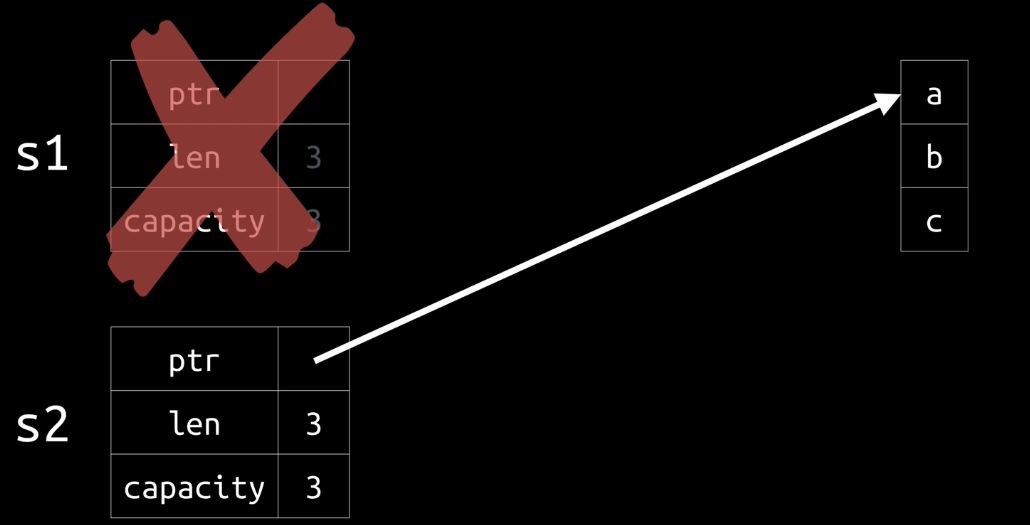
\includegraphics[width=3in]{screenshots/2022-07-16T19-12-15Z.png} 
 \end{figure}

\begin{itemize}
  \item We could still use s1 if it was \textbf{mut} and assign it a new value,
    but here, \textbf{immutable}, makes it like \textbf{garbage collector} 
\end{itemize}

\begin{tcolorbox}[title=If we don't to move but to copy the value,colback=backcolour,size=small,left=4mm]
\begin{lstlisting}[language=rust]
let s1 = String::from("abc");
let s2 = s1.clone(); //makes a copy of s1
\end{lstlisting}
\end{tcolorbox}

\begin{itemize}
  \item \textbf{Clone} instead of \textbf{copy} : Clone performs the same initial copy
    \textbf{but} then it \textbf{also} copies the \textbf{heap date} and adjust's s2's pointer to it 
    \item Stack + Heap = Value 
    \item Copy only means stack data copy, heap data and pointer updates requires \textbf{cloning} $\equiv $ deep copy 
    \item \textbf{Value dropping} :
      \begin{enumerate}
        \item Run Destructor, immediatly 
        \item Free heap, immediatly 
        \item Pop stack, immediatly
      \end{enumerate}
\end{itemize}

\begin{tcolorbox}[title=Another move situation,colback=backcolour,size=small,left=4mm]
\begin{lstlisting}[language=rust]
let s1 = String::from("abc");

fn do_stuff(s: String) {
  //do stuff, returns nothing
}

do_stuff(s1); // s1 gets moved into the local variable "s" in do_stuff(), we cannot use s1 anymore

// to fix that, we could move it back
let mut s1 = String::from("abc"); 
s1 do_stuff(s1); // s gets moved back out of the function
print..s1..; error
fn do_stuff(s: String) -> String { // add return type 
  s // returns s
}
//Not a usual pattern !

// usually the function consummes the past in value
// For more often cases we should use References

\end{lstlisting}
\end{tcolorbox}

\section{References and Borrowing}

Instead of moving our variable, let's use a reference
\begin{tcolorbox}[colback=backcolour,size=small,left=4mm]
\begin{lstlisting}[language=rust]
let s1 = String::from("abc");
do_stuff(&s1); // we pass a reference to s1, do stuff no borrows a reference to the value

fn do_stuff(s: &String) { // the & indicates a reference to a type
}
\end{lstlisting}
\end{tcolorbox}

\begin{itemize}
  \item A \textbf{reference} allows a variable to \textbf{retain the ownership} of its value. Only the reference gets  moved into the function 
  \item At the \textbf{end} of func, the ref goes out of scope and gets \textbf{dropped}. The borrowing \textbf{ends} 
  \item When we create a ref to s1, rust creates a ptr to s1, rust handles their creation and destruction. \textbf{References are only ptr}
  \item \textbf{Lifetimes} is a rule that \textbf{references must always be valid}, compiler wont let the creation of a reference of the data it is referencing, and no pointing to null 
  \item References defaults to \textbf{immutable} 
\end{itemize}


\begin{tcolorbox}[title=Mut ref to a mut value,colback=backcolour,size=small,left=4mm]
\begin{lstlisting}[language=rust]
let mut s1 = String::from("abc");
do_stuff(&s1); // *1
do_stuff(&mut s1); // *2

fn do_stuff(s: &String) {
  s.insert_str(0, "Hi, "); // ERROR with *1 , not with *2
  }
// now we can use ref to CHANGE the value as well
\end{lstlisting}
\end{tcolorbox}

\begin{itemize}
  \item We did not have to dereference the mutable reference in order to alter it in the do\_stuff ? 
  \item We use the same .method to access String method on a ref than we do on the value itself
    $\rightarrow$ the dot operator \textbf{auto-dereferences} down to the actual value 
  \item \textbf{Manually deref} is done by (*ref) it is required by most other operators like the \textbf{assigment} $\rightarrow$ read from or write from the actual value 
  \item This does apply to types, i32 $\rightarrow$ \&i32 and \&mut i32 
  \item x: \&mut i32 If our variable is a \textbf{mut ref} to a value, then deref x would give \textbf{mut} access to a value and the opposite.. 
  \item Since ref are implemented via \textbf{ptr}, rust has a rule to stay safe :
    We can always have \textbf{one mut ref} and \textbf{any \# of immutable refs}, applying across \textbf{all threads}  
\end{itemize}

\begin{figure}[H] 
	 \centering 
	 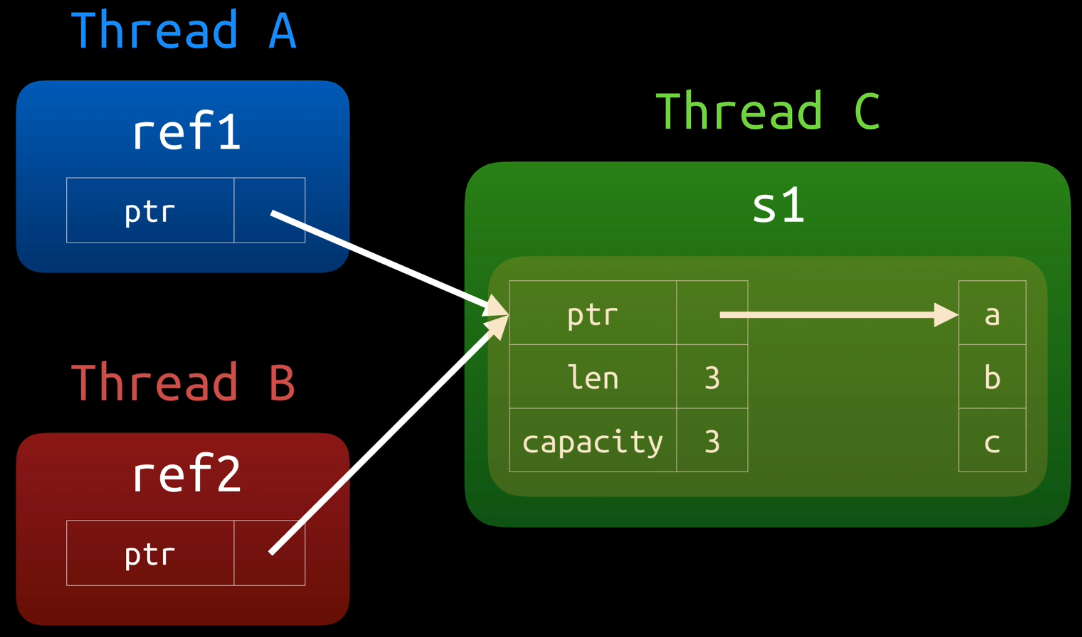
\includegraphics[width=2in]{screenshots/2022-07-16T21-38-55Z.png} 
 \end{figure}

\begin{itemize}
  \item All this rules are enforced by the compiler 
\end{itemize}


\end{multicols*}


\chapter{The Meat Of Rust}

\begin{multicols*}{2}

\begin{itemize}
  \item Structs $\equiv $ Classes 
  \item Can have [data fiels, methods, associated funcs] 
  \item Naming like \textit{AnExample} : capital-camel case 
\end{itemize}

\begin{tcolorbox}[title=Syntax,colback=backcolour,size=small,left=4mm]
\begin{lstlisting}[language=rust]
struct RedFox {
  enemy: bool,
  life: u8, // we can end the last field with "," too !
  }
\end{lstlisting}
\end{tcolorbox}

\begin{tcolorbox}[title=Init Struct,colback=backcolour,size=small,left=4mm]
\begin{lstlisting}[language=rust]
// verbose, you need to specify a value for every single field
let fox = RedFox {
  enemy: true,
  life: 70,
  }; 
// typically we implement an associated func to use as a constructor to create a struct with default values and then call that
impl RedFox {
  fn new() -> Self { // this is an associated func because it does not have a form of self as its first param
    Self { // both Self here refers to RedFox, we could also use it 
      enemy: true,
      life: 70,
    }
  }
}
\end{lstlisting}
\end{tcolorbox}

\begin{itemize}
  \item Methods and Funcs are def in an \textbf{impl}ementation block separate from the struct definition 
  \item \textbf{new} is a conventional name for creating a struct with \textbf{default values} 
  \item \textbf{Self} can be used in place of the struct name inside the implementation block 
\end{itemize}

\begin{tcolorbox}[title=Creating,colback=backcolour,size=small,left=4mm]
\begin{lstlisting}[language=rust]
let fox = RedFox::new(); // :: accesses a associated func in the struct
// once values are instantiated, dot syntax is used
let life_left = fox.life;
fox.enemy = false;
fox.some_method();
\end{lstlisting}
\end{tcolorbox}
\begin{itemize}
  \item "::" is the scope operator, used to \textbf{access} parts of the \textbf{namespace-like} things
\end{itemize}

\begin{tcolorbox}[title=Defining Methods,colback=backcolour,size=small,left=4mm]
\begin{lstlisting}[language=rust]
impl RedFox { // also in the impl block
  // assoc functions
  fn function()
  // methods
  fn move(self)
  fn borrow(&self)
  fn mut_borrow(&mut self)
  }
\end{lstlisting}
\end{tcolorbox}

\begin{itemize}
  \item Methods always take some form of \textbf{self} as arg 
  \item There is no struct \textbf{inheritance}, because we have \textbf{Traits}
\end{itemize}

\section{Traits}

\begin{itemize}
  \item Similar to interfaces in other lang, composition $>$ inheritance 
  \item \textbf{Traits} define required behaviour, functions and methods that a struct
    must implement if it wants to have that trait
\end{itemize}

\begin{tcolorbox}[title=Example,colback=backcolour,size=small,left=4mm]
\begin{lstlisting}[language=rust]
stuct RedFox {
  enemy: bool,
  life: u32,
  }
trait Noisy {
  fn get_noise(&self) -> &str; // specifies that the struct must have a method named get_noise() returning a borrowed string slice if the struct wants to be Noisy
  }

impl Noisy for RefFox {
  fn get_noise(&self) -> &str { "Meow?" }
  } // our implementation of the get_noise method is "meow"

// Why bother doing this instead of just implementing it directly without traits ?
// Once we have trait involved, we can start writing generic functions that accept any value implementing the trait
fn print_noise<T: Noisy>(item: T) {
  println!("{}", item.get_noise());
  } // this func takes an item of type T defined to be anything that implements the Noisy trait
  // the func can use any behaviour on item that Noisy trait defines
  // This generic function can take any type as long as it satisfies the noisy trait

  // as long as one of either the trait or stuct is defined, we can implement any trait for any struct, including builtin or import types from other packages

impl Noisy for u8 {
  fn get_noise(&self) -> &str { "Byte!" }
  }

fn main() {
  print_noise(5_u8); // prints "Byte!"
  }
\end{lstlisting}
\end{tcolorbox}

\begin{itemize}
  \item Special trait called \textbf{Copy}, if our type implements copy, then it will be \textbf{copied} instead of \textbf{moved} in move situation,
    makes sense for small values fitting entirely on the stack, explaining why \textbf{simple primitive types} like int, floats and booleans implement Copy. If a type uses the \textbf{heap} then it cannot implement \textbf{Copy}. We can opt-in to impl Copy with our own types only if
    our type only uses other Copy types. 
  \item Traits implement \textbf{inheritance}
\end{itemize}

\begin{figure}[H] 
	 \centering 
	 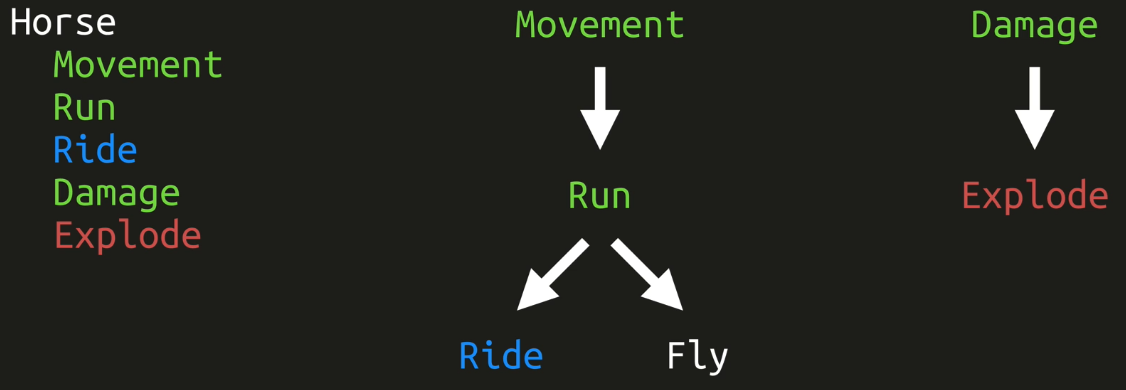
\includegraphics[width=2.5in]{screenshots/2022-07-17T11-58-25Z.png} 
 \end{figure}


\begin{tcolorbox}[title=Traits can also have default behaviours,colback=backcolour,size=small,left=4mm]
\begin{lstlisting}[language=rust]
trait Run {
  fn run(&self) {
    println!("I'm Running !")
  }
}

struct Robot {}
impl Run for Robot {} // does not overwrite the default run method

// fully functional example

fn main() {
  let robot = Robot {};
  robot.run();
  }
\end{lstlisting}
\end{tcolorbox}

\begin{itemize}
  \item \textbf{Cannot define Fields} as part of traits, the workaround is to define setter and getter methods in our trait 
\end{itemize}

\section{Collections}

\begin{itemize}
  \item The following \textbf{collections} are all in the \textbf{std}
  \item \textbf{Vec<T>} : Vector holds a \textbf{bunch of one type}, useful in place of lists or arrays in other lang, most common, they have a \textbf{ton of methods} [insert, remove, split, splice, sort, repeat, binary search,..]
\end{itemize}

\begin{tcolorbox}[title=Examples,colback=backcolour,size=small,left=4mm]
\begin{lstlisting}[language=rust]
let mut v: Vec<i32> = Vec::new(); // vector creation
v.push(2); // once we have it, we can push some values into it, acts like stack
v.push(4);
let x = v.pop(); // x is 4
println!("{}", v[0]) // "2"

// macro vec! Creating vectors from literal values
let mut v = vec![2, 4, 6];
\end{lstlisting}
\end{tcolorbox}

\begin{itemize}
  \item \textbf{HashMap<K, V>} generic collection where we specify \textbf{type} for \textbf{key} and \textbf{value} $\equiv $ dictionary 
  \item Its point is to be able to insert, look up, remove values by key in constant time
\end{itemize}

\begin{tcolorbox}[title=Examples,colback=backcolour,size=small,left=4mm]
\begin{lstlisting}[language=rust]
let mut h: HashMap<u8, bool> = HashMap::new();
h.insert(5, true);
h.insert(6, false);
let have_five = h.remove(&5).unwrap(); // we use remove() to get a value, remove() returns an enum called Option
\end{lstlisting}
\end{tcolorbox}

There are a bunch of other collections :
\begin{itemize}
  \item \textbf{VecDeque} uses a ring buffer to implement a double-ended queue, able to efficiently add or remove items from the front and the back,
    but everything else is less efficient than a regular Vec 
  \item \textbf{LinkedList} has the dubious distinction of being quick at adding or removing items at an arbitrary point in the list, but slow doing anything else
  \item \textbf{HashSet} Hashing implementation of a set, performing set operations efficiently 
  \item \textbf{BinaryHeap} is like a priority queue which always pops off the max value
  \item \textbf{BTreeMap and BTreeSet} are alternate map and set impl using a modified binary tree, \textbf{usecase} over other hash variants if mapping keys or set values to always be sorted is needed
\end{itemize}


\section{Enums}

\begin{itemize}
  \item \textbf{Enums} $\equiv $ \textbf{Algebraic Data Types}
\end{itemize}

\begin{tcolorbox}[title=Syntax,colback=backcolour,size=small,left=4mm]
\begin{lstlisting}[language=rust]
enum Color { // capital-camel case
  Red, // names of the variants
  Green,
  Blue,
  }
let color = Color::Red;
\end{lstlisting}
\end{tcolorbox}

Top code works but The real power of rust enums comes from \textbf{associating data and methods with the variants}

\begin{tcolorbox}[colback=backcolour,size=small,left=4mm]
\begin{lstlisting}[language=rust]
enum DispenserItem { 
  Empty, // we can always have a named variant with no data
  Ammo(u8), // variant can have a single type of data
  Things(String, i32) // a tuple
  Place {x: i32, y: i32}, // an anonymous struct of data
}

use DispenserItem::*;
let item = Empty;
//or 
let item = Things("hat".to_string(), 7);
// or...
// we can impl functions and method for enum
// we could use enum for generics
\end{lstlisting}
\end{tcolorbox}

\begin{tcolorbox}[title=Option Enum (Std),colback=backcolour,size=small,left=4mm]
\begin{lstlisting}[language=rust]
// We will use this one all the time
enum Option<T> { // T means any type, we could use any other valid identifier, but the idiomatic thing in rust is to use T or other CAP letter
  Some(T),
  None,
  } // option enum represents when something is present or not, useful when we want to reach of null or nil
  // you either have some value wrapped in the Some variant or None
\end{lstlisting}
\end{tcolorbox}

\begin{tcolorbox}[title=Examples,colback=backcolour,size=small,left=4mm]
\begin{lstlisting}[language=rust]
if let Some(x) = my_variable {
  println!("Value is {}", x);
  }
// enums can represent any data, we need to use patters to examine them
// to check for a single variant, we use the "if let" expression
// if let : takes pattern that will match one of those variants
// if pattern match => cond true => var inside the pattern are created
// Great for one variant but not to handle all at once => Match expr
\end{lstlisting}
\end{tcolorbox}

\begin{tcolorbox}[title=Match Expression,colback=backcolour,size=small,left=4mm]
\begin{lstlisting}[language=rust]
match my_variable {
  Some(x) => {
    println!("value is {}", x); // most of the time blocks
  },
  Some(x) => x.squared() + 1, // but func call works too
  None => {
    println!("no value :(");
  },
}
_ => { .. // _ is a pattern that match everything, use for default or "anything else" branch

// we could use the return value of that match expr but don't forget the ; at the end

\end{lstlisting}
\end{tcolorbox}

\begin{itemize}
  \item The pattern in a match expression \textbf{must be exhaustive} 
  \item Either \textbf{all} branch need to return Nothing or all need to return the Same type
\end{itemize}

In depth : \textbf{Option} and \textbf{Result} : they are use all over the std !

\subsection{Option}%
\label{sub:Option}

\begin{tcolorbox}[colback=backcolour,size=small,left=4mm]
\begin{lstlisting}[language=rust]
enum Option<T> {
  Some(T),
  None,
  }  // options is used whenever something might be absent

// to create a non variant to an option
let mut x: Option<i32> = None;
// since option and variants are used so much, they're already included in the std prelude, no need to "use"
x = Some(5); // using option with a concrete type makes the comp infer the type => we can leave off the declaration Option<i32>
x.is_some(); // true => if x is the Some variant
x.is_none(); // false

for i in x {
  println!("{}", i);
  } // option impl the IntoIterator trait, so can be treated as a vector of 0 or 1 items 
\end{lstlisting}
\end{tcolorbox}

\subsection{Result}%
\label{sub:Result}

\begin{itemize}
  \item Result is used whenever something might have a useful result or an error 
  \item Appears a lot in the io module
\end{itemize}

\begin{tcolorbox}[title=Definition,colback=backcolour,size=small,left=4mm]
\begin{lstlisting}[language=rust]
#[must_use] // makes it a compiler warning to silent drop a result
enum Result<T, E> { // both types are generic but independent
  Ok(T),
  Err(E),
}
\end{lstlisting}
\end{tcolorbox}

\begin{tcolorbox}[title=Example,colback=backcolour,size=small,left=4mm]
\begin{lstlisting}[language=rust]
use std::fs::File;

fn main() {
  File::open("foo");
} // this returns a result since the file might not get opened successfully

// Simplest way to handle error
fn main() {
  let res = File::open("foo");
  //
  let f = res.unwrap(); // if the result is an Ok then this gives out the wanted file struct, if error, then this crashes to program
  //
  let f = res.expect("error message"); // unwrap + crash output message
  }

// just like Option, there are helper methods like is_ok and is_err

fn main() {
  let res = File::open("foo");
if res.is_ok() {
  let f = res.unwrap(); // here unwrap will never crash
  }
}
// can also do pattern matching
  match res {
    Ok(f) => {/* */},
    Err(e) => {/* */},
  }
\end{lstlisting}
\end{tcolorbox}


\section{Closures}

\begin{itemize}
  \item \textbf{Closures} are encountered when we want to \textbf{spawn a thread}, or do \textbf{functional programming} with iterators and in some other common places in the std 
  \item It's an anonymous func that can borrow or capture data from the scope it is \textbf{nested} in
  \item types of args and return value are all inferred from how we use the argument and what we return
\end{itemize}

\begin{tcolorbox}[title=Syntax,colback=backcolour,size=small,left=4mm]
\begin{lstlisting}[language=rust]
let add = |x, y| { x + y } // this creates a callable closure

add(1, 2); // returns 3

// we could have no parameters
|| { x + y } // the block too but useless
// a closure will borrow a ref to values in the enclosing scope

\end{lstlisting}
\end{tcolorbox}

\begin{tcolorbox}[title=Example of closure borrowing,colback=backcolour,size=small,left=4mm]
\begin{lstlisting}[language=rust]
let s = "<emoji>".to_string();
let f = || {
  println!("{}", s);
};

f(); // prints <emoji>
// this is great if our closure never outlives the variable it is referencing,
// but the compiler won't let us send this over to another thread because it might longer than this thread
// Fortunately, closures support move semantics, so we can force to move any var it uses into itself and take ownership of them
let f = move || { // now s in owned by the closure, it'll live until death of the closure
\end{lstlisting}
\end{tcolorbox}

\begin{tcolorbox}[title=Functionnal Programming Example,colback=backcolour,size=small,left=4mm]
\begin{lstlisting}[language=rust]
let mut = vec![2, 4, 6];

v.iter() // get vector iterator, now we have lots of methods using closures available
  .map(|x| x * 3) // multiply each item by 3
  .filter(|x| *x > 10) // discard any value not greater than 10
  .fold(0, |acc, x| acc + x); // with initial value and closure to sum remaining values together
\end{lstlisting}
\end{tcolorbox}


\section{Threads}

\begin{itemize}
  \item Rust threading is \textbf{portable}
\end{itemize}

\begin{tcolorbox}[title=Fully functional example,colback=backcolour,size=small,left=4mm]
\begin{lstlisting}[language=rust]
use std::thread;

fn main() {
  let handle = thread::spawn(move || { // thread::spawn takes closure w/o args, closure gets exec as the main function of the thread
    // do stuff in a child thread, common practice is to call a function here
  });
  // do stuff simultaneously in the main thread

  // wait until thread has exited
  handle.join().unwrap(); // spawn returns a join handle, we can call it, ant it'll pause the thread that we're joining has completed and exited
  }
\end{lstlisting}
\end{tcolorbox}

\begin{itemize}
  \item The spawned thread could have an error or a panic, or could return a value successfully back to the thread that joins it 
  \item What we get from the \textbf{join call} is a result that \textbf{wraps} a possible success value returned from the thread or an error if thread panic 
  \item Treading is heavyweight. Creating a new one allocates an os-dependent amount of RAM for the thread's own stack, often mb's. 
    Whenever a CPU switches from running one thread to another, it has to do an expensive context switch. the \textbf{More threads} sharing same CPU core = the \textbf{More overhead} we'll have in context switching 
    \item Threads are a fantastic tool when cpu and memory are needed concurrently $\rightarrow$ They can run simultaneously on multi cores and do more work 
    \item However if we are just waiting for something like disk, network io, then look into \textbf{async/await} 
\end{itemize}

\end{multicols*}

\end{document}
